\documentclass[class=article, crop=false]{standalone}
\usepackage{my_preamble}
\begin{document}
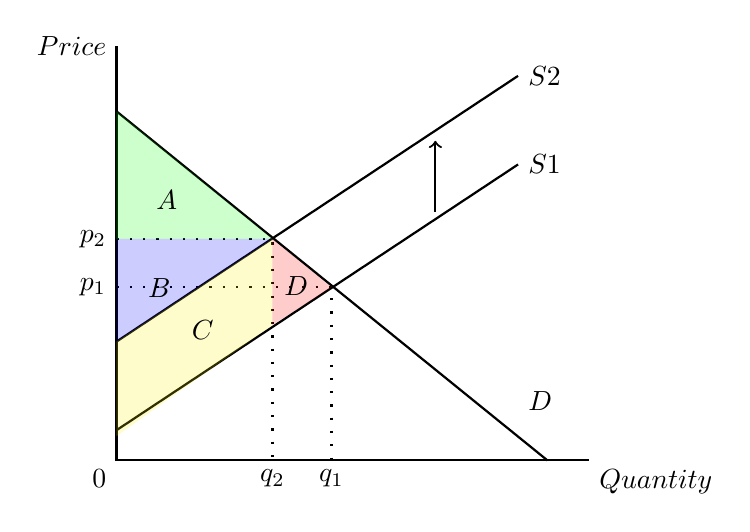
\begin{tikzpicture}[thick,font=\sffamily,scale=1.5]

	 \draw (0,3.5) node[left]{$Price$} -- (0,0) node[below left] {$0$} -- (4,0) node[below right]{$Quantity$}; %labels
	\draw plot[domain=0:3.65,smooth] (\x,2.95-0.81*\x); %Demand
	\draw[] (0,0.25) -- (3.4,2.5); %S1
	\draw[] (0,1) -- (3.4,3.25); %S2
	
	%dotted lines
	 \draw[loosely dotted] (0,1.46) node[left]{$p_{1}$} -| node[pos=0.25,below=3mm] {} (1.82,0) node[below]{$q_{1}$}; %equib 1
	 \draw[loosely dotted] (0,1.87) node[left]{$p_{2}$} -| node[pos=0.25,below=3mm] {} (1.32,0) node[below]{$q_{2}$}; %equib 2
	 
	 %fill
	\fill [fill=green, fill opacity=0.2] (0,2.95) node[left]{} -- (0,1.87) node[below left] {} -- (1.32,1.87) node[below left] {}; %green fill
	\fill [fill=blue, fill opacity=0.2] (0,1.87) node[left]{} -- (0,1) node[below left] {} -- (1.32,1.87) node[below left] {}; %blue fill
	\fill [fill=yellow, fill opacity=0.2] (0,1) node[left]{} -- (0,0.2) node[below left] {} -- (1.32,1.14) node[below left] {} -- (1.32,1.87) node[below left] {}; %yellow fill
	\fill [fill=red, fill opacity=0.2] (1.32,1.87) node[left]{} -- (1.82,1.46) node[below left] {} -- (1.32,1.14) node[below left] {}; %red fill
	
	%labels and arrows 
	\node[right] at (3.4,0.5) {$D$}; %Demand label
	\node[right] at (3.4,2.5) {$S1$}; %s1 label
	\node[right] at (3.4,3.25) {$S2$}; %s2 label
	
	\node[right] at (0.25,2.2) {$A$}; %A label
	\node[right] at (0.18,1.45) {$B$}; %B label
	\node[right] at (0.55,1.1) {$C$}; %C label
	\node[left] at (1.71,1.47) {$D$}; %D label
	 
	\draw [->] (2.7,2.1) -- (2.7,2.7); %x arrow
\end{tikzpicture}
\end{document}